\documentclass{yann}
\usepackage{tikz}
\usetikzlibrary{matrix,calc}

\newcommand\sqn[2]{\ccro{1,#1}×\ccro{1,#2}}
\newcommand\MM[1]{\M{M}{#1}{𝕂}}
\newcommand\BC{\mathscr{C}}

\begin{document}
\title{Algèbre linéaire 2}
\maketitle

\Para{Notations}
$𝕂$ désigne un corps;
toutes les matrices considérées seront à coefficients dans $𝕂$;
tous les £evs. considérés seront des £Kevdfs..

% ---------------------------------------------------------------------------
\section{Matrice}

% ---------------------------------------------------------------------------
\subsection{Définition algébrique}

\Para{Définition}

Soit $(n,p)∈ℕ_*^2$.
Une \emph{matrice} de type $(n,p)$ est une application de $\sqn np$ dans $𝕂$.
L'ensemble des matrices de type $(n,p)$ est noté $\MM{n,p}$.
La matrice $M \colon (i,j) \mapsto m_{i,j}$ est notée $M = \pa{ m_{i,j} }_{\substack{1≤i≤n\\1≤j≤p}}$.

\Para{Opérations}

\begin{enumerate}
\item
  Si $A$ et $B$ sont deux matrices de type $(n,p)$,
  on définit la matrice $C = A+B$ de type $(n,p)$
  par $c_{i,j} = a_{i,j} + b_{i,j}$
  pour tout $(i,j)∈\sqn np$.
\item
  Si $λ$ est un scalaire et $A$ une matrice de type $(n,p)$,
  on définit la matrice $B = λA$ de type $(n,p)$
  par $b_{i,j} = λa_{i,j}$ pour tout $(i,j)∈\sqn np$.
\item
  Si $A$ est une matrice de type $(n,p)$ et $B$ est une matrice de type $(p,q)$,
  on définit la matrice $C = A × B$ de type $(n,q)$
  par \[ c_{i,j} = ∑_{k=1}^p a_{i,k} b_{k,j} \] pour tout $(i,j)∈\sqn nq$.
\end{enumerate}

\Para{Propriétés}

\begin{enumerate}
\item
  $(\MM{n,p},+,⋅)$ est un £ev..
\item
  Si $A ∈ \MM{n,p}$, $B ∈ \MM{p,q}$ et $C ∈ \MM{q,r}$, alors
  les produits suivants sont bien définis
  et $(A × B) × C = A × (B × C)$.
\item
  Si $λ∈ 𝕂$, $A ∈ \MM{n,p}$ et $B ∈ \MM{p,q}$,
  alors $(λA) × B = A × (λB) = λ(A × B)$.
\item
  Si $A ∈ \MM{n,p}$, $B ∈ \MM{n,p}$ et $C ∈ \MM{p,q}$,
  alors les sommes et les produits suivants sont bien définis
  et $(A + B) × C = A×C + B×C$.
\item
  Si $A ∈ \MM{n,p}$, $B ∈ \MM{p,q}$ et $C ∈ \MM{p,q}$,
  alors les sommes et les produits suivants sont bien définis
  et $A × (B + C) = A×B + A×C$.
\end{enumerate}

\Para{Remarque}

En général $A × B ≠ B × A$, même dans le cas de deux matrices $(n,n)$.

% ---------------------------------------------------------------------------
\subsection{Lien avec les £evs.}

\Para{Définition: coordonnées d'un vecteur}

Soit $E$ un £Kev. de dimension $n$ et $\B = \nUplet e1n$ une base de $E$.
On sait que tout vecteur $x∈E$ se décompose de façon unique sous la forme
$x = ξ_1 e_1 + \dots + ξ_n e_n$ où $\nUplet ξ1n ∈ 𝕂^n$
On appelle coordonnées de $x$ dans la base $E$ le $n$-uplet
\[ \Coords_\B(x) = \nUplet ξ1n ∈𝕂^n. \]

\Para{Remarque}

On identifiera fréquemment les $n$-uplets avec les matrices colonnes;
cela est légitime car l'application
\[ \Fonction{ϕ}{𝕂^n}{\MM{n,1}}{\nUpletξ1n}{\Matrix{ξ_1;\vdots;ξ_n}} \]
est un isomorphisme.

\Para{Définition: matrice d'un endomorphisme}

Soit $E$ et $F$ deux £evdfs., $\B = \nUplet e1p$ une base de $E$ et $\B' = \nUplet f1n$ une base de $F$.
Pour tout $j∈\ccro{1,p}$, le vecteur $u(e_j)$ se décompose dans la base $\B'$:
\[ u(e_j) = ∑_{i=1}^n a_{i,j} f_i. \]
On appelle \emph{matrice de l'endomorphisme $u$} la matrice suivante, de type $(n,p)$:
\[ \Mat(u,\B \to \B') = \Mat_{\B\to\B'}(u) = \bigPa{ a_{i,j} }_{\substack{1≤i≤n\\1≤j≤p}}. \]
\begin{center}
  \begin{tikzpicture}[
      every left delimiter/.style={xshift=0.75em},
      every right delimiter/.style={xshift=-0.75em},
      dots/.style={
        line width=1pt,
        line cap=round,
        dash pattern=on 0pt off 5pt,
        shorten >=.1cm,
    shorten <=.1cm}]
    \matrix (M) [
      matrix of nodes,
      left delimiter=(,
      right delimiter=),
    ]{
      \node (A) {$a_{1,1}$}; &[1.1cm] \node (B) {$a_{1,p}$}; \\[1.1cm]
      \node (C) {$a_{n,1}$}; &        \node (D) {$a_{n,p}$}; \\
    };

    \draw (M.west) node[left] {$\Mat\limits_{\B\to\B'}(u)=$};
    \draw [dots] (A.east)  -- (B.west);
    \draw [dots] (C.east)  -- (D.west);
    \draw [dots] (A.south) -- (C.north);
    \draw [dots] (B.south) -- (D.north);
    \draw (A) [yshift=0.7cm] node (E) {$u(e_1)$};
    \draw (B) [yshift=0.7cm] node (F) {$u(e_p)$};
    \draw (B) [xshift=1cm]   node (G) {$f_1$};
    \draw (D) [xshift=1cm]   node (H) {$f_n$};
    \draw [dots] (E.east)  -- (F.west);
    \draw [dots] (G.south) -- (H.north);
  \end{tikzpicture}
\end{center}
Dans le cas où $E=F$ et $\B=\B'$, on la note $\Mat(u,\B)$ ou $\Mat_\B(u)$.

\Para{Définition}

Inversement, si l'on se donne une matrice $M ∈ \MM{n,p}$,
on peut définir une application linéaire, dite \emph{canoniquement associée à $M$}, par
\[ \Fonction{f_M}{𝕂^p}{𝕂^n}{x}{Mx} \]
où l'on identifie $𝕂^n$ et $\MM{n,1}$ ainsi que $𝕂^p$ et $\MM{p,1}$.

Si l'on note $\B$ la base canonique de $𝕂^p$ et $\B'$ la base canonique de $𝕂^n$,
on vérifie facilement que
\[ \Mat(f_M, \B \to \B') = M. \]

\Para{Théorème}

Soit $E$ et $F$ deux £evdfs. munis de bases $\B$ et $\B'$.
Soit $\Fn uEF$ une application linéaire et $x$ un vecteur de $E$.
Alors \[ \Coords_{\B'}\bigPa{u(x)} = \Mat_{\B\to\B'}(u) × \Coords_\B(x). \]

\Para{Théorème}

Soit $E$ et $F$ deux £evdfs. munis de bases $\B$ et $\B'$.
L'application
\[ \Fonction{}{\mathscr{L}(E,F)}{\MM{n,p}}{u}{\Mat_{\B\to\B'}(u)} \]
est linéaire et bijective, autrement dit un isomorphisme.

\Para{Théorème}

Soit $E$, $F$, $G$ trois £evdfs. munis des bases respectives $\B$, $\B'$ et $\B''$.
Soit $\Fn uEF$ et $\Fn vFG$ deux applications linéaires.
Alors
\[ \Mat_{\B\to\B''}(v◦u) = \Mat_{\B'\to\B''}(v) ×\Mat_{\B\to\B'}(u). \]

% ---------------------------------------------------------------------------
\subsection{Formules de changement de base}

\Para{Définition}

Soit $E$ un £evdf., $\B$ et $\B'$ deux bases de $E$.
On appelle \emph{matrice de passage} de $\B$ à $\B'$ la matrice
\[ \Pass(\B\to\B') = \Mat_{\B'\to\B}(\Id_E). \]

De façon plus explicite, notons $\B = \nUplet e1n$,
$\B' = \nUplet f1n$ et $\Pass(\B\to\B') = \bigPa{ a_{i,j} }$.
Dans ce cas, on a
\[ ∀j ∈ \ccro{1,n} \+ f_j = ∑_{i=1}^n a_{i,j} e_i. \]
Ainsi,
\begin{center}
  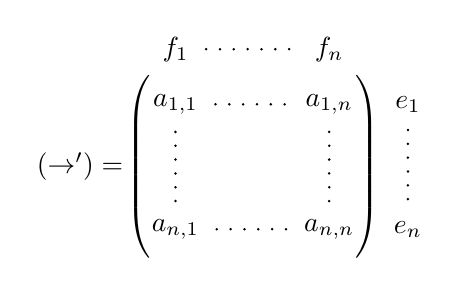
\begin{tikzpicture}[
      every left delimiter/.style={xshift=0.75em},
      every right delimiter/.style={xshift=-0.75em},
      dots/.style={
        line width=1pt,
        line cap=round,
        dash pattern=on 0pt off 5pt,
        shorten >=.1cm,
    shorten <=.1cm}]
    \matrix (M) [
      matrix of nodes,
      left delimiter=(,
      right delimiter=),
    ]{
      \node (A) {$a_{1,1}$}; &[1.1cm] \node (B) {$a_{1,n}$}; \\[1.1cm]
      \node (C) {$a_{n,1}$}; &        \node (D) {$a_{n,n}$}; \\
    };

    \draw (M.west) node[left] {$\Pass(\B\to\B')=$};
    \draw [dots] (A.east)  -- (B.west);
    \draw [dots] (C.east)  -- (D.west);
    \draw [dots] (A.south) -- (C.north);
    \draw [dots] (B.south) -- (D.north);
    \draw (A) [yshift=0.7cm] node (E) {$f_1$};
    \draw (B) [yshift=0.7cm] node (F) {$f_n$};
    \draw (B) [xshift=1cm]   node (G) {$e_1$};
    \draw (D) [xshift=1cm]   node (H) {$e_n$};
    \draw [dots] (E.east)  -- (F.west);
    \draw [dots] (G.south) -- (H.north);
  \end{tikzpicture}
\end{center}

\Para{Proposition}

Soit $E$ un £evdf. et $\B$, $\B'$ et $\B''$ trois bases de $E$.
Alors
\begin{enumerate}
\item
  $\Pass(\B \to \B') × \Pass(\B' \to \B'') = \Pass(\B \to \B'')$;
\item
  $\Pass(\B \to \B')$ est inversible, et son inverse est $\Pass(\B' \to \B)$.
\end{enumerate}


\Para{Proposition}

Soit $E$ un £evdf., $\B$ et $\B'$ deux bases de $E$.
Soit $x$ un vecteur de $E$.
Alors \[ X = PX'\]
où
\begin{itemize}
\item $P = \Pass(\B \to \B')$,
\item $X = \Coords_\B(x)$,
\item $X' = \Coords_{\B'}(x)$.
\end{itemize}

\Para{Proposition}

Soit $E$ un £evdf. muni de deux bases $\B$ et $\B'$.
Soit $F$ un £evdf. muni de deux bases $\BC$ et $\BC'$.
Soit $\Fn uEF$ une application linéaire.
Alors on a \[ A' = Q^{-1} A P \]
où
\begin{itemize}
\item $P = \Pass(\B \to \B')$,
\item $Q = \Pass(\BC \to \BC')$,
\item $A = \Mat_{\B \to \BC}(u)$,
\item $A' = \Mat_{\B' \to \BC'}(u)$.
\end{itemize}

\Para{Corollaire}

Soit $E$ un £evdf. muni de deux bases $\B$ et $\B'$.
Soit $u$ un endomorphisme de $E$.
Alors on a \[ A' = P^{-1} A P \]
où
\begin{itemize}
\item $P = \Pass(\B \to \B')$,
\item $A = \Mat_{\B}(u)$,
\item $A' = \Mat_{\B'}(u)$.
\end{itemize}

% ------------------------------------------------------------------------------
\section{Matrices carrés}

\subsection{Matrices inversibles}

%\Para{Définition}

La \emph{matrice identité} de taille $n$ est la matrice
$I_n = \bigPa{ δ_{i,j} } ∈ \MnK$.

\Para{Théorème}

Soit $A$ et $B$ deux matrices carrées de taille $n$.
On suppose que $AB = I_n$.
Alors $BA = I_n$.

% ---------------------------------------------------------------------------
\subsection{Similitude}

\Para{Définition}

Soit $A$ et $B$ deux matrices carrées de $\MnK$.
On dit que $A$ et $B$ sont \emph{semblables}
£ssil. existe une matrice inversible $P∈\GLnK$
telle que \[ B = P^{-1} A P. \]


\Para{Propriétés}

Il s'agit d'une relation d'équivalence, £cad.:
\begin{enumerate}
\item $A \sim A$;
\item si $A \sim B$, alors $B \sim A$;
\item si $A \sim B$ et $B \sim C$, alors $A \sim C$.
\end{enumerate}

\Para{Proposition}

Soit $u$ un endomorphisme de $E$.
Les matrices $\Mat_\B(u)$ et $\Mat_{\B'}(u)$ sont semblables.

\Para{Proposition}

Soit $A$ et $B$ deux matrices.
Soit $E$ un £ev. de dimension $n$ et $\B$ une base de $E$.
Notons $u$ l'unique endomorphisme de $E$ tel que $\Mat_\B(u) = A$.
Alors $A$ et $B$ sont semblables £ssi. il existe une base $\B'$ de $E$ telle que $\Mat_{\B'}(u) = B$.

% ------------------------------------------------------------------------------
\subsection{Trace}

\Para{Définition}

Soit $A = \bigl(a_{i,j}\bigr)_{1≤i,j≤n}∈\MnK$ une matrice carrée.
La \emph{trace} de la $A$ est le scalaire
\[ \Tr(A) = ∑_{k=1}^n a_{k,k}. \]

\Para{Propriétés}

\begin{enumerate}
\item La trace est une application linéaire de $\MnK$ dans $𝕂$.
  Autrement dit, pour toutes matrices $(A,B)∈\MnK^2$ et pour tous $(λ,μ)∈𝕂^2$, on a
  \[ \Tr(λA + μB) = λ\Tr(A) + μ\Tr(B). \]
\item Pour toutes matrices $(A,B) ∈\MnK^2$, on a
  \[ \Tr(AB) = \Tr(BA). \]
\item Si $A$ et $B$ sont deux matrices semblables de $\MnK$, alors elles ont la même trace.
\end{enumerate}

\Para{Attention}

En général, $\Tr(ABC)≠\Tr(ACB)$.

\Para{Définition}[trace d'un endomorphisme]

Soit $E$ un $𝕂$-espace vectoriel de dimension finie et $u$ un endomorphisme de $E$.
Soit $\B$ une base de $E$ et $M$ la matrice de $u$ dans la base $\B$.
La quantité $\Tr(M)$ ne dépendant pas du choix de la base $\B$, mais seulement de $u$, on l'appelle \emph{trace} de l'endomorphisme $u$ et on note $\Tr(u) = \Tr(M)$.

\Para{Propriétés}

\begin{enumerate}
\item La trace est une application linéaire de $\LE$ dans $𝕂$.
\item Si $u$ et $v$ sont deux endomorphismes de $E$, alors $\Tr(u◦v) = \Tr(v◦u)$.
\end{enumerate}

% ---------------------------------------------------------------------------
\subsection{Déterminants}

\Para{Théorème}

Soit $n∈\Ns$.
Il existe une unique application $\Fn{d}{\MnK}{𝕂}$ vérifiant les propriétés suivantes:
\begin{enumerate}
\item
  $d(I_n) = 1$;
\item
  $d(A) = 0$ si deux colonnes de $A$ sont égales;
\item
  Si on fixe $n-1$ colonnes de $A$, l'application qui à la dernière colonne associe $d(A)$ est linéaire.

  Plus précisément, soit $A$, $B$ et $C$ des matrices de $\MnK$.
  pour $1≤j≤n$, on note $A_j$, $B_j$ et $C_j$ les $j$-ème colonnes de $A$, $B$ et $C$ respectivement.
  On suppose que
  \begin{itemize}
  \item $A_k = λB_k + μC_k$ où $k ∈ \ccro{1,n}$ et $(λ,μ)∈𝕂^2$;
  \item pour tout $j ∈ \ccro{1,n} ∖ \acco{k}$, $A_j = B_j = C_j$.
  \end{itemize}
  Alors $d(A) = λd(B) + μd(C)$.
\end{enumerate}

Cette application $d$ vérifie alors automatiquement les propriétés suivantes:
\begin{enumerate}[resume]
\item
  $d(B) = -d(A)$ si $B$ se déduit de $A$ en échangeant deux colonnes;
\item
  $d(B) = d(A)$ si $B$ se déduit de $A$ par une opération du type $C_i \leftarrow C_i + ∑_{k≠i} α_k C_k$;
\item
  $d(B) = λd(A)$ si $B$ se déduit de $A$ par une opération du type $C_i \leftarrow λC_i$;
\item
  $d(A) = d(\T A)$ pour toute matrice $A∈\MnK$;
\item
  dans toutes les propriétés précédentes, on peut remplacer \enquote{colonnes} par \enquote{lignes};
\item
  $d(AB) = d(A) d(B)$ pour toutes les matrices $(A,B)∈\MnK^2$;
\item
  $d(A) ≠ 0$ £ssi. $A$ est inversible.
\end{enumerate}

% ---------------------------------------------------------------------------
\subsubsection{Déterminant de Vandermonde}

\Para{Définitions}

Soit $\nUplet a1n ∈𝕂^n$.
La \emph{matrice de Vandermonde} associée à $\nUplet a1n$ est
\[ M = \begin{pmatrix}
    1 &  1 &  1 &  \dots &  1  \\
    a_1 &  a_2 &  a_3 &  \dots &  a_n  \\
    a_1^2 &  a_2^2 &  a_3^2 &  \dots &  a_n^2  \\
    \vdots &  \vdots &  \vdots &   &  \vdots  \\
a_1^{n-1} &  a_2^{n-1} &  a_3^{n-1} &  \dots &  a_n^{n-1}  \end{pmatrix}. \]
Le \emph{déterminant de Vandermonde} $V \nUplet a1n$ est le déterminant de la matrice de Vandermonde ci-dessus.

\Para{Théorème}

Avec les mêmes notations,
\[ V\nUplet a1n = ∏_{1≤i < j≤n} (a_j - a_i). \]
En particulier,
\begin{itemize}
\item $V(a) = 1$,
\item $V(a,b) = b-a$,
\item $V(a,b,c) = (b-a)(c-a)(c-b)$.
\end{itemize}

\Para{Corollaire}

La matrice de Vandermonde associée à $\nUplet a1n$ est inversible si et seulement si les nombres $\nUplet a1n$ sont deux à deux distincts.

% ---------------------------------------------------------------------------
\section{Matrices par blocs}

\Para{Définition}

Soit $(s,t) ∈(\Ns)^2$, $(n_1, \dots, n_s) ∈(\Ns)^s$ et $(p_1, \dots, p_t) ∈(\Ns)^t$ des entiers naturels non nuls.
On pose:
\begin{itemize}
\item pour tout $k ∈\Dcro{0,s}$, $σ_k = ∑_{i=1}^k n_i$,
\item pour tout $l ∈\Dcro{0,t}$, $τ_l = ∑_{j=1}^l p_j$,
\item $n = n_1 + \dots + n_s = σ_s$,
\item $p = p_1 + \dots + p_t = τ_t$.
\end{itemize}

Soit $A∈\mathrm{M}_{n,p}(𝕂) = \bigl( a_{ij} \bigr)_{\substack{1≤i≤n \\ 1≤j≤p}}$ une matrice.
Sa décomposition par blocs suivant le découpage $\nUplet n1s$ pour les lignes et $\nUplet p1t$ pour les colonnes est
\begin{center}
  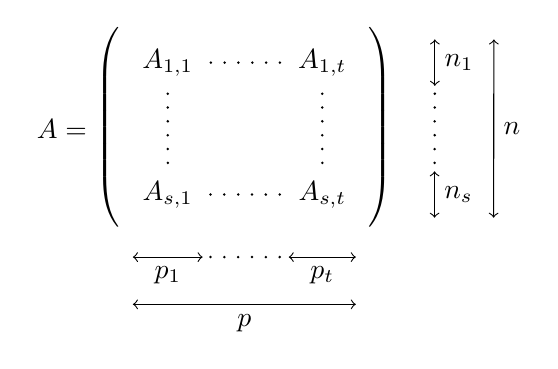
\begin{tikzpicture}[
      dots/.style={
        line width=1pt,
        line cap=round,
        dash pattern=on 0pt off 5pt,
        shorten >=.1cm,
    shorten <=.1cm}]
    \matrix[
      matrix of nodes,
      left delimiter=(,
      right delimiter=),
    ]{
      \node (A) {$A_{1,1}$}; &[1.1cm] \node (B) {$A_{1,t}$}; \\[1.1cm]
      \node (C) {$A_{s,1}$}; &        \node (D) {$A_{s,t}$}; \\
    };

    \draw [dots] (A.east)  -- (B.west);
    \draw [dots] (C.east)  -- (D.west);
    \draw [dots] (A.south) -- (C.north);
    \draw [dots] (B.south) -- (D.north);

    \draw [<->]  ([xshift=1cm]B.north east) -- node [right] {$n_1$} ([xshift=1cm]B.south east);
    \draw [<->]  ([xshift=1cm]D.north east) -- node [right] {$n_s$} ([xshift=1cm]D.south east);
    \draw [dots] ([xshift=1cm]B.south east) -- ([xshift=1cm]D.north east);
    \draw [<->]  ([xshift=1.75cm]B.north east) -- node [right] {$n$} ([xshift=1.75cm]D.south east);

    \draw [<->]  ([yshift=-0.5cm]C.south west) -- node [below] {$p_1$}([yshift=-0.5cm]C.south east);
    \draw [<->]  ([yshift=-0.5cm]D.south west) -- node [below] {$p_t$}([yshift=-0.5cm]D.south east);
    \draw [dots] ([yshift=-0.5cm]C.south east) -- ([yshift=-0.5cm]D.south west);
    \draw [<->]  ([yshift=-1.1cm]C.south west) -- node [below] {$p$} ([yshift=-1.1cm]D.south east);

    \node[xshift=-0.9cm] at ($(A.west)!0.5!(C.west)$) { $A =$ };
  \end{tikzpicture}
\end{center}
où pour tout $k∈\Dcro{1,s}$ et $l∈\Dcro{1,t}$, on a
\[ A_{k,l} = \begin{pmatrix}
    a_{1+σ_{k-1},1+τ_{l-1}}  &  \dots &  a_{1+σ_{k-1},τ_l}  \\
    \vdots &   &  \vdots  \\
    a_{σ_k, 1+τ_{l-1}} &  \dots &  a_{σ_k,τ_l}
\end{pmatrix} ∈\mathrm{M}_{n_k,q_l}(𝕂). \]

\Para{Proposition}[addition par blocs]

Soit $A$ et $B$ deux matrices de $\mathrm{M}_{n,p}(𝕂)$ exprimées par blocs selon les mêmes découpages. Soit $(λ,μ)∈𝕂^2$.
Alors la matrice $λA + μB$ s'exprime par blocs selon les mêmes découpages que $A$ et $B$, et les blocs s'obtiennent en combinant les blocs situés aux mêmes places.

\Para{Théorème}[produit par blocs]

Soit $A∈\mathrm{M}_{n,p}(𝕂)$ et $B∈\mathrm{M}_{p,q}(𝕂)$.
On suppose que $A$ a une décompositon par blocs suivant le découpage $\nUplet n1s$ pour les lignes et $\nUplet p1t$ pour les colonnes.
On suppose que $B$ a une décomposition par blocs suivant le découpage $\nUplet p1t$ pour les lignes et $\nUplet q1u$ pour les colonnes.

Alors le produit $C = AB∈\mathrm{M}_{n,q}(𝕂)$ admet une décomposition par blocs suivant le découpage $\nUplet n1s$ pour les lignes et $\nUplet q1u$ pour les colonnes
\[ C = \begin{pmatrix} C_{1,1} &  \dots &  C_{1,u}  \\  \vdots &   &  \vdots  \\  C_{s,1} &  \dots &  C_{s,u} \end{pmatrix} \]
où pour tous $i∈\Dcro{1,s}$ et $j∈\Dcro{1,u}$,
\[ C_{i,j} = ∑_{k=1}^t A_{i,k} B_{k,j} \]

\Para{Remarque}

Le cas qui nous intéressera le plus fréquemment est celui des matrices carrées ayant le même découpage pour les lignes et pour les colonnes. Dans ce cas, les blocs diagonaux sont également des matrices carrées.

\Para{Proposition}

Soit $E$ un espace vectoriel de dimension finie $n$, $F$ un sous-espace vectoriel de $E$ et $u∈\LE$.
Soit $\B' = \nUplet e1p$ une base de $F$ telle que $\B = \nUplet e1n$ soit une base de $E$.
Soit $A$ la matrice de l'endomorphisme $u$ dans la base $\B$;
on la décompose par blocs selon le découpage $(p,n-p)$ pour les lignes et les colonnes:
\[ A = \Matrix{A_{1,1}, A_{1,2}; A_{2,1}, A_{2,2}}. \]
Alors $F$ est stable par $u$ si et seulement si ma matrice $A_{2,1}$ est nulle.
Dans ce cas, notons $v$ l'endomophisme induit par $u$ sur $F$.
La matrice de $v$ dans la base $\B'$ est $A_{1,1}$.

% ---------------------------------------------------------------------------
\subsection{Déterminants par blocs}

\Para{Attention}

Si $A$, $B$, $C$ et $D$ sont des matrices de $\MnK$ et si
$M = \begin{pmatrix} A & B \\ C & D \end{pmatrix} ∈\mathrm{M}_{2n}(𝕂)$, alors en général
\[ \det(M) ≠\det(AD-BC). \]

\Para{Théorème}[déterminant triangulaire par blocs]

Soit $A∈\MnK$ une matrice carrée admettant une décomposition par blocs suivant le découpage $\nUplet n1s$ pour les lignes et pour les colonnes.
On note $A = \bigl( A_{i,j} \bigr)_{1≤i,j≤s}$ cette décomposition, de sorte que $A_{i,j}∈\mathrm{M}_{n_i,n_j}(𝕂)$.
On suppose que $A$ est triangulaire supérieure par blocs, £cad. que
\[ ∀(i,j)∈\Dcro{1,s}^2 \+ i > j \implies A_{i,j} = 0. \]

Alors le déterminant de $A$ est égal au produit des déterminants des blocs diagonaux:
\[ \det(A) = ∏_{k=1}^s \det(A_{k,k}). \]

Le résultat est identique dans le cas des matrices triangulaires inférieures par blocs.

% ---------------------------------------------------------------------------
\section{Divers}

\subsection{Polynôme de matrice}

\Para{Définition}

Soit $A∈\MnK$ une matrice carrée.
On définit par récurrence $A^n$ pour $n∈ℕ$ par
$A^0 = I_n$ et $∀n∈ℕ$, $A^{n+1} = A×A^n$.

Pour $P = ∑_{k=0}^d a_k X^k$, on pose $P(A) = ∑_{k=0}^d a_k A^k$.

\Para{Proposition}

Soit $E$ un $𝕂$-espace vectoriel de dimension finie, $\B$ une base de $E$, $u∈\LE$,
$A = \Mat_\B(u)$ et $P∈𝕂[X]$.

Alors $\Mat_\B P(u) = P(A)$.

\Para{Corollaire}

Soit $A∈\MnK$.
L'application \[ \Fonction{ϕ_A}{𝕂[X]}{\MnK}{P}{P(A)} \]
est également un morphisme d'algèbre.
Autrement dit, si $P$ et $Q$ sont deux polynômes et $λ$ un scalaire, on a
\begin{enumerate}
\item $(λP)(A) = λP(A)$
\item $(P+Q)(A) = P(A) + Q(A)$
\item $(PQ)(A) = P(A)×Q(A)$
\end{enumerate}

\Para{Proposition}

Soit $A∈\MnK$, $Q∈\GLnK$ et $P∈𝕂[X]$.
Alors
\[ P \bigl( Q^{-1}AQ \bigr) = Q^{-1} \, P(A) \, Q. \]

% ---------------------------------------------------------------------------
\section{Exercices}

\Exercice

Soit $E = ℝ_3[X]$ et $\B$ la base canonique.
Soit $f∈\LE$ défini par $f(P) = P(X+1)$.
\begin{enumerate}
\item Déterminer $A = \Mat_\B f$.
\item Montrer que $A$ est inversible et calculer $A^{-1}$.
\item Reprendre les questions précédentes pour $E=ℝ_n[X]$.
\end{enumerate}

\Exercice

Soit $A = \begin{pmatrix} -2 & 1 & 1 \\ 8 & 1 & -5 \\ 4 & 3 & -3 \end{pmatrix}$
et $C = \begin{pmatrix} 1 & 2 & -1 \\ 2 & -1 & -1 \\ -5 & 0 & 3 \end{pmatrix}$.

Existe-t-il une matrice $B$ telle que $A=BC$?

\Exercice

Soit $E$ un $𝕂$-£evdf. tel que $f◦f = -\Id_E$.
Montrer qu'il existe une base $\B$ telle que la matrice de $f$ dans cette base soit diagonale par blocs, de la forme $\Mat_\B f = \mathrm{diag}(A,A,\dots,A)$ où $A = \begin{pmatrix} 0 & -1 \\ 1 & 0 \end{pmatrix}$.

\Exercice[matrices à diagonale dominante]

Soit $A∈\MnC$ telle que
\[ ∀i∈\Dcro{1,n} \+ ∑_{\substack{1≤j≤n \\ j≠i}} \Abs{a_{i,j}} < \Abs{a_{i,i}}. \]
Montrer que $A$ est inversible. On pourra montrer que $\Ker A = \Acco{0}$.

\Exercice

Soit $a∈ℝ$.
Pour $n∈ℕ^*$, on définit le déterminant d'ordre $n$
\[ Δ_n = \begin{vmatrix}
    a &  1 &  0 &  \cdots &  0  \\
    1 &  a &  1 &  \ddots &  \vdots  \\
    0 &  1 &  a &  \ddots &  0  \\
    \vdots &  \ddots &  \ddots &  \ddots &  1  \\
0 &  \cdots &  0 &  1 &  a \end{vmatrix} \]
\begin{enumerate}
\item Déterminer une relation de récurrence linéaire d'ordre 2 vérifiée par la suite $(Δ_n)$.
\item On suppose $a = 2\cosθ$ où $θ∈\intO{0,π}$.
  Montrer que \[ Δ_n = \frac{\sin\bigl((n+1)θ\bigr)}{\sinθ}. \]
\end{enumerate}

\Exercice

Soit $A∈\MnC$. On pose
\[ \Fonction{φ}{\MnC}{\MnC}{M}{-M + \Tr(M)A.} \]
\begin{enumerate}
\item Montrer que $φ$ est un endomorphisme de $\MnC$.
\item À quelle condition $φ$ est-il un isomorphisme?
\item Soit $B∈\MnC$.
  Déterminer l'ensemble des solutions de l'équation $φ(M)=B$.
\end{enumerate}

\Exercice

Soit $A$, $B$, $C$, $D$ des matrices carrées de $\MnK$.
On suppose que $CD = DC$ et que $D$ est inversible.
\begin{enumerate}
\item
  En considérant le produit par blocs
  \[ \Matrix{I_n,-BD^{-1};0,I_n} \Matrix{A,B;C,D} \]
  montrer que
  \[ \det \Matrix{A,B;C,D} = \det(AD-BC). \]
\item Montrer que cette dernière formule est encore vraie si l'on ne suppose plus que $D$ est inversible.
\item Trouver un contre-exemple si l'on ne suppose plus que $C$ et $D$ commutent.
\end{enumerate}

\end{document}
